\chapter{Software Installation}
\label{sec::A_si}
Since all of the software is freely available on GitHub, you can always find a build section within the provided readme file there. The links to the respective GitHub folders are provided within each following section. For the case of an error that may occur during the build procedure, do no hesitate to open up an issue there. I will then help you to get the software running on your device.
\section{Build the Pattern Generator}
\label{sec::A1_pg}
The pattern generator can be found on GitHub at the following \href{https://github.com/mhubii/nmpc_pattern_generator}{link}. Proceed as described below.
\begin{enumerate}
	\item 
\end{enumerate}
\section{Build the Android Joystick App}
\label{sec::A2_aa}
The Joystick app can be found on GitHub at the following \href{https://github.com/mhubii/ijoy}{link}. Proceed as described below.
\begin{enumerate}
	\item Clone the Android app from GitHub with
	\newline \inlinecode{}{git clone https://github.com/mhubii/ijoy.git}
	\item Copy the \inlinecode{}{.apk} file that you cloned from GitHub to your Android smartphone.
	\item Make sure your device allows installation of apps from unknown sources. Under Android 7:
	\subitem Go to settings and open lock \inlinecode{}{screen\&security}.
	\subitem Find entry \inlinecode{}{unkown sources} and enable it.
	\item Find the \inlinecode{}{.apk} using the file browser of your choice and execute it (figure \ref{fig::A2_apk} (a) and (b)).
	\begin{figure}[h]
		\centering
		\subcaptionbox{File browser.}%
		[.22\linewidth]{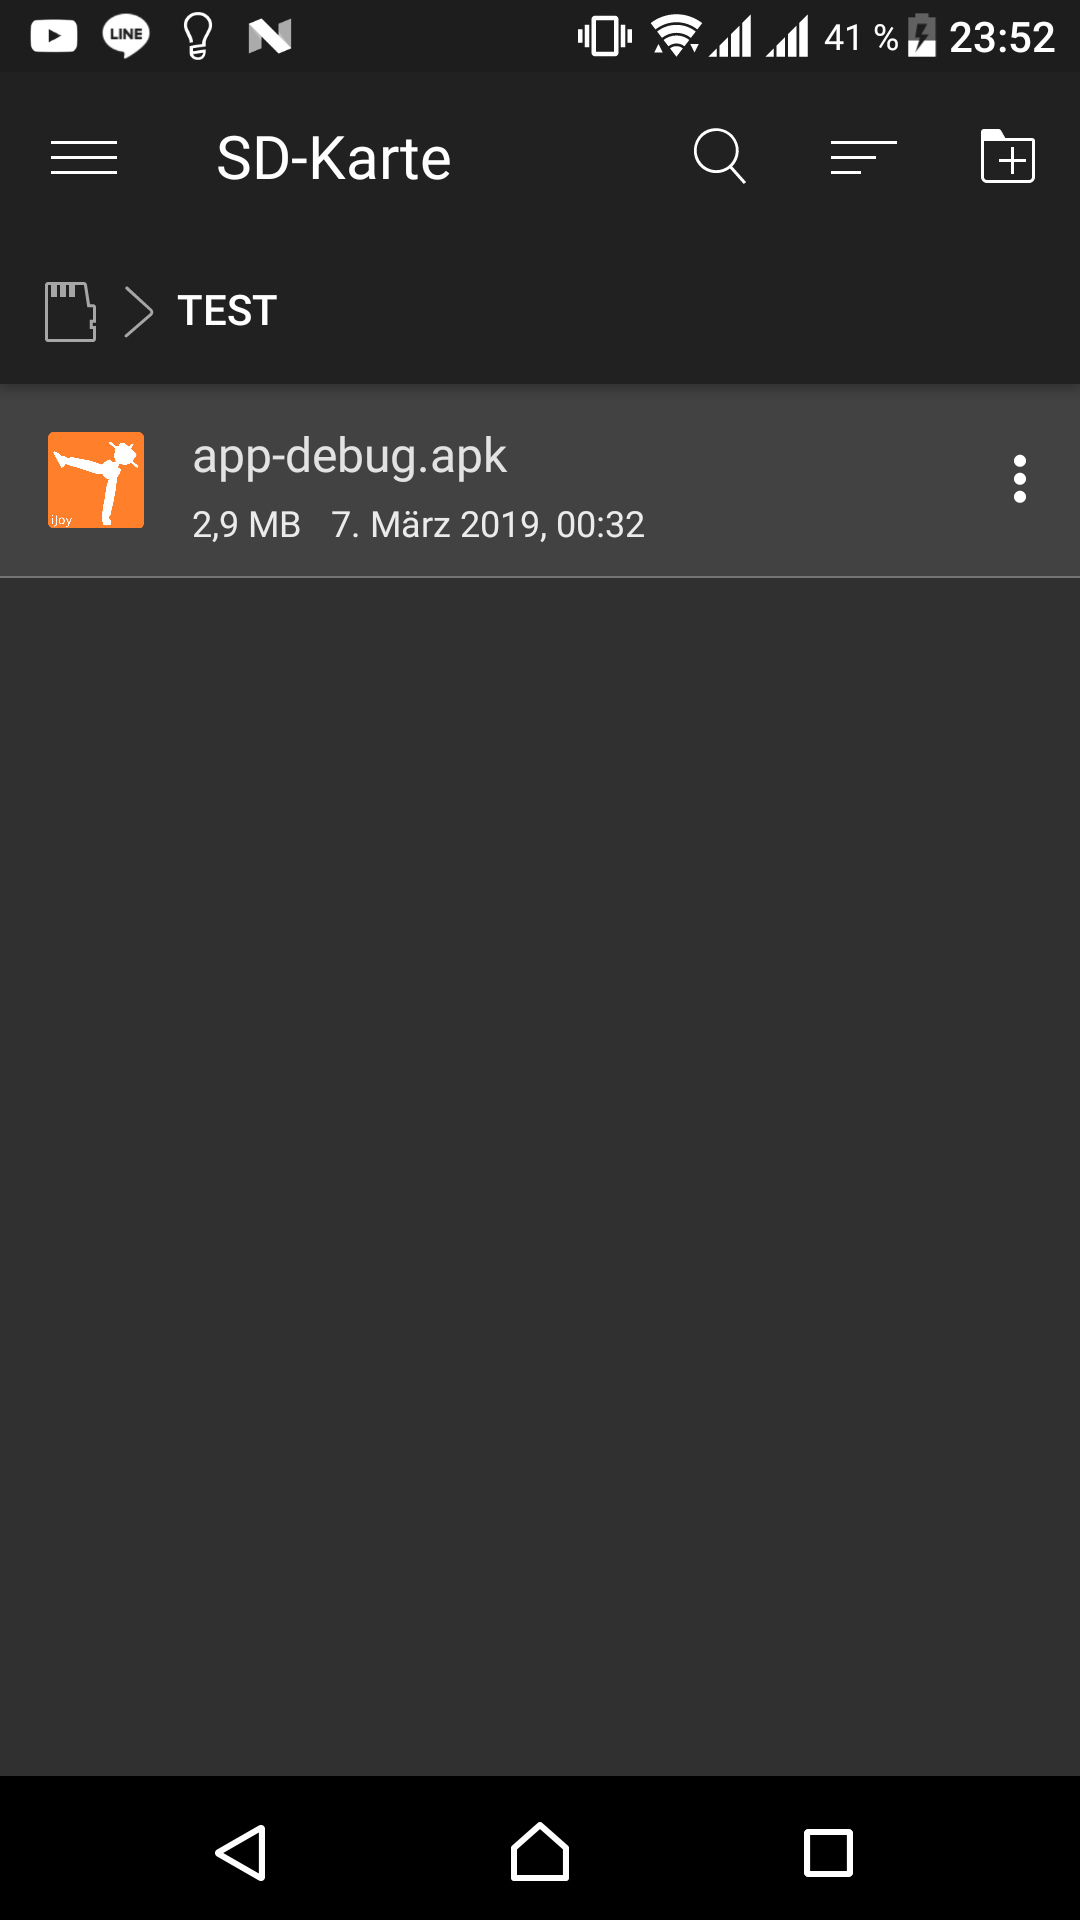
\includegraphics[scale=.06]{chapters/07_appendix/img/file_browser.png}}
		\subcaptionbox{Menu.}%
		[.22\linewidth]{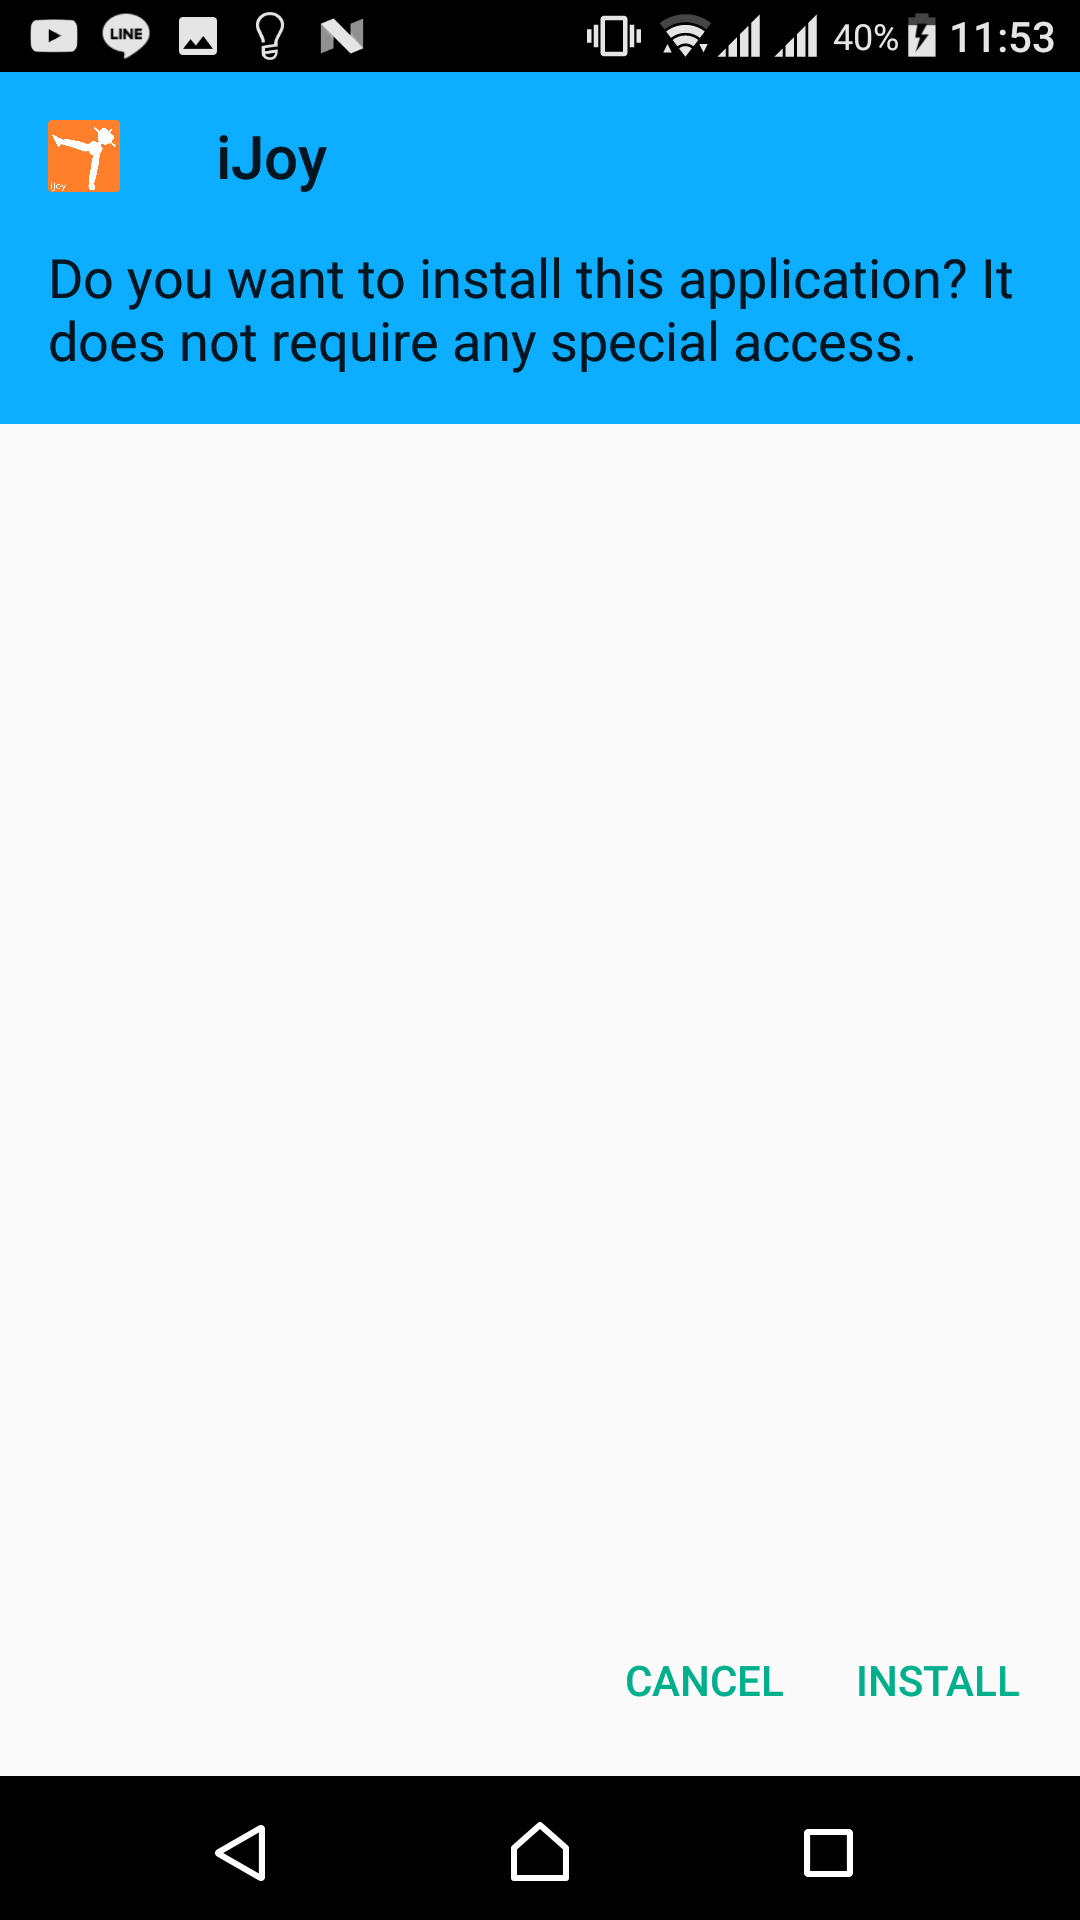
\includegraphics[scale=.06]{chapters/07_appendix/img/installation_start.png}}
		\subcaptionbox{Installing.}%
		[.22\linewidth]{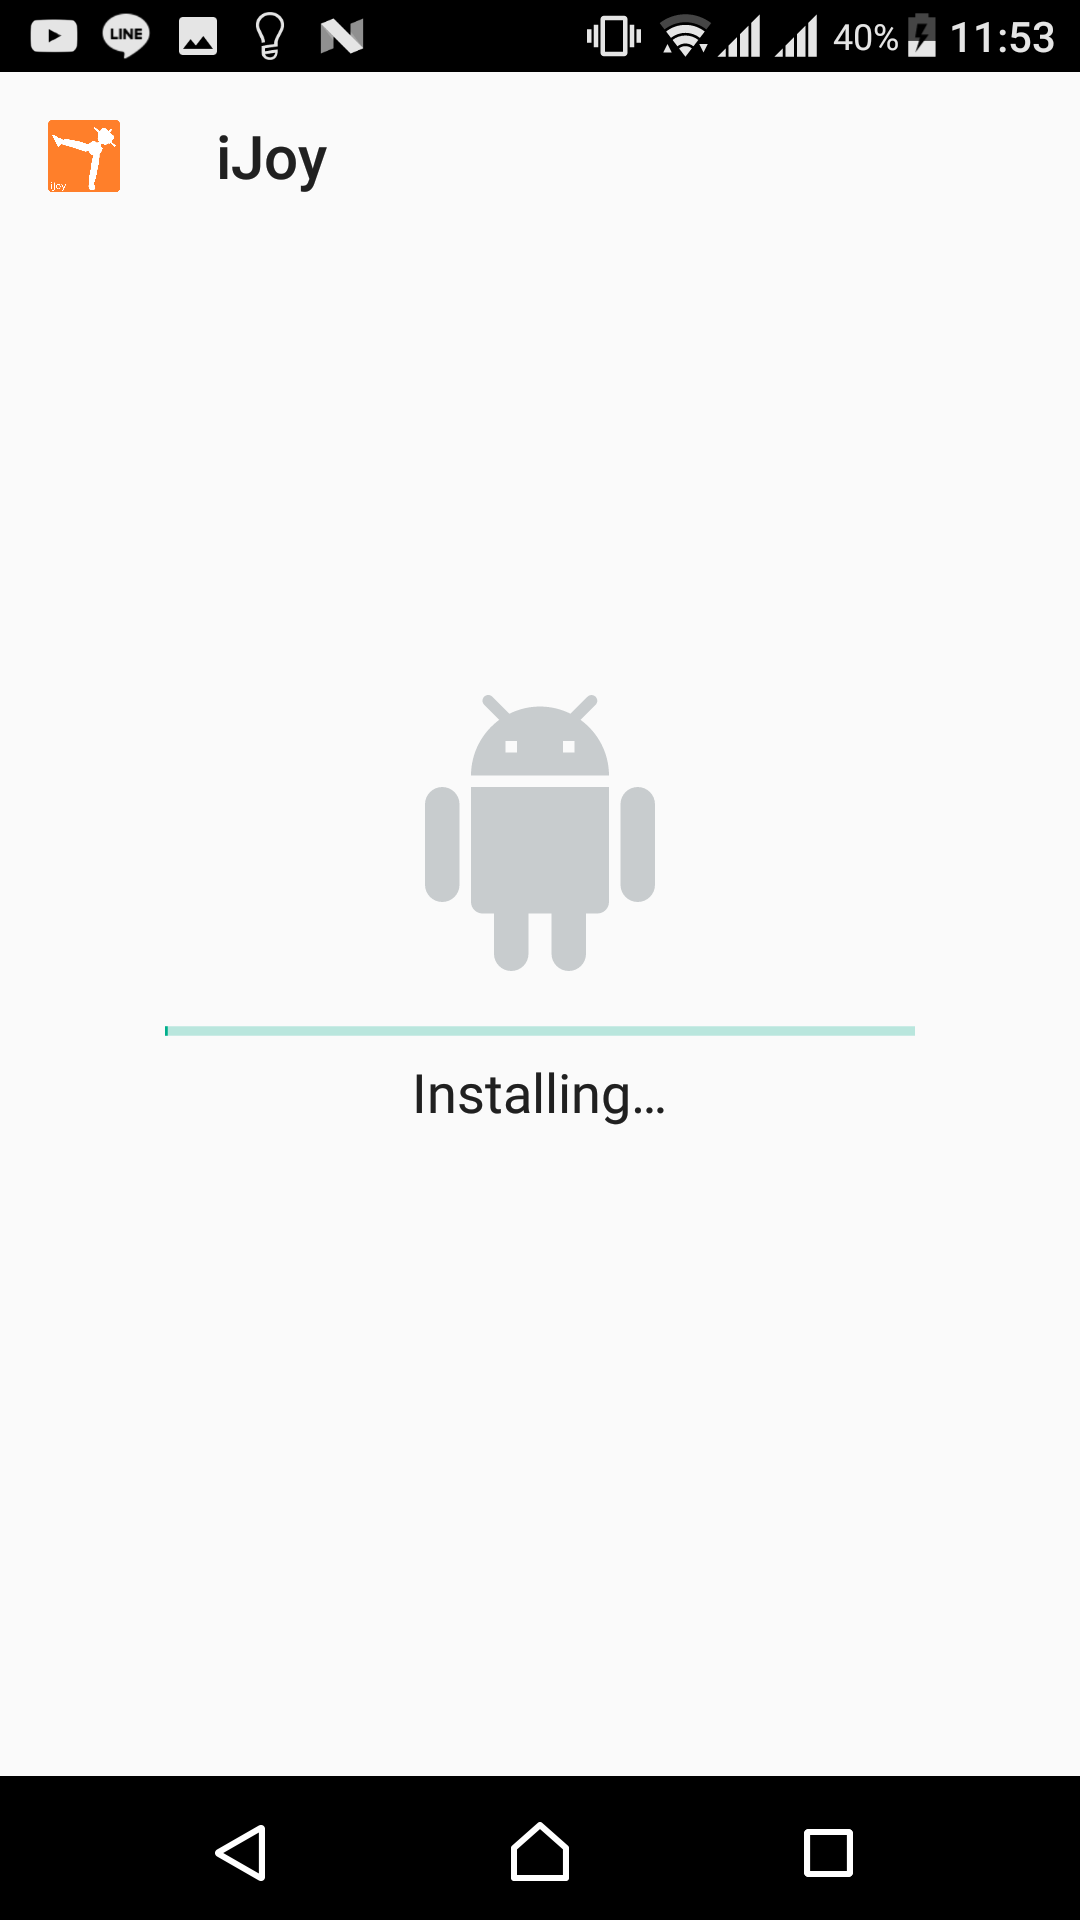
\includegraphics[scale=.06]{chapters/07_appendix/img/installation.png}}
		\subcaptionbox{Finished.}%
		[.22\linewidth]{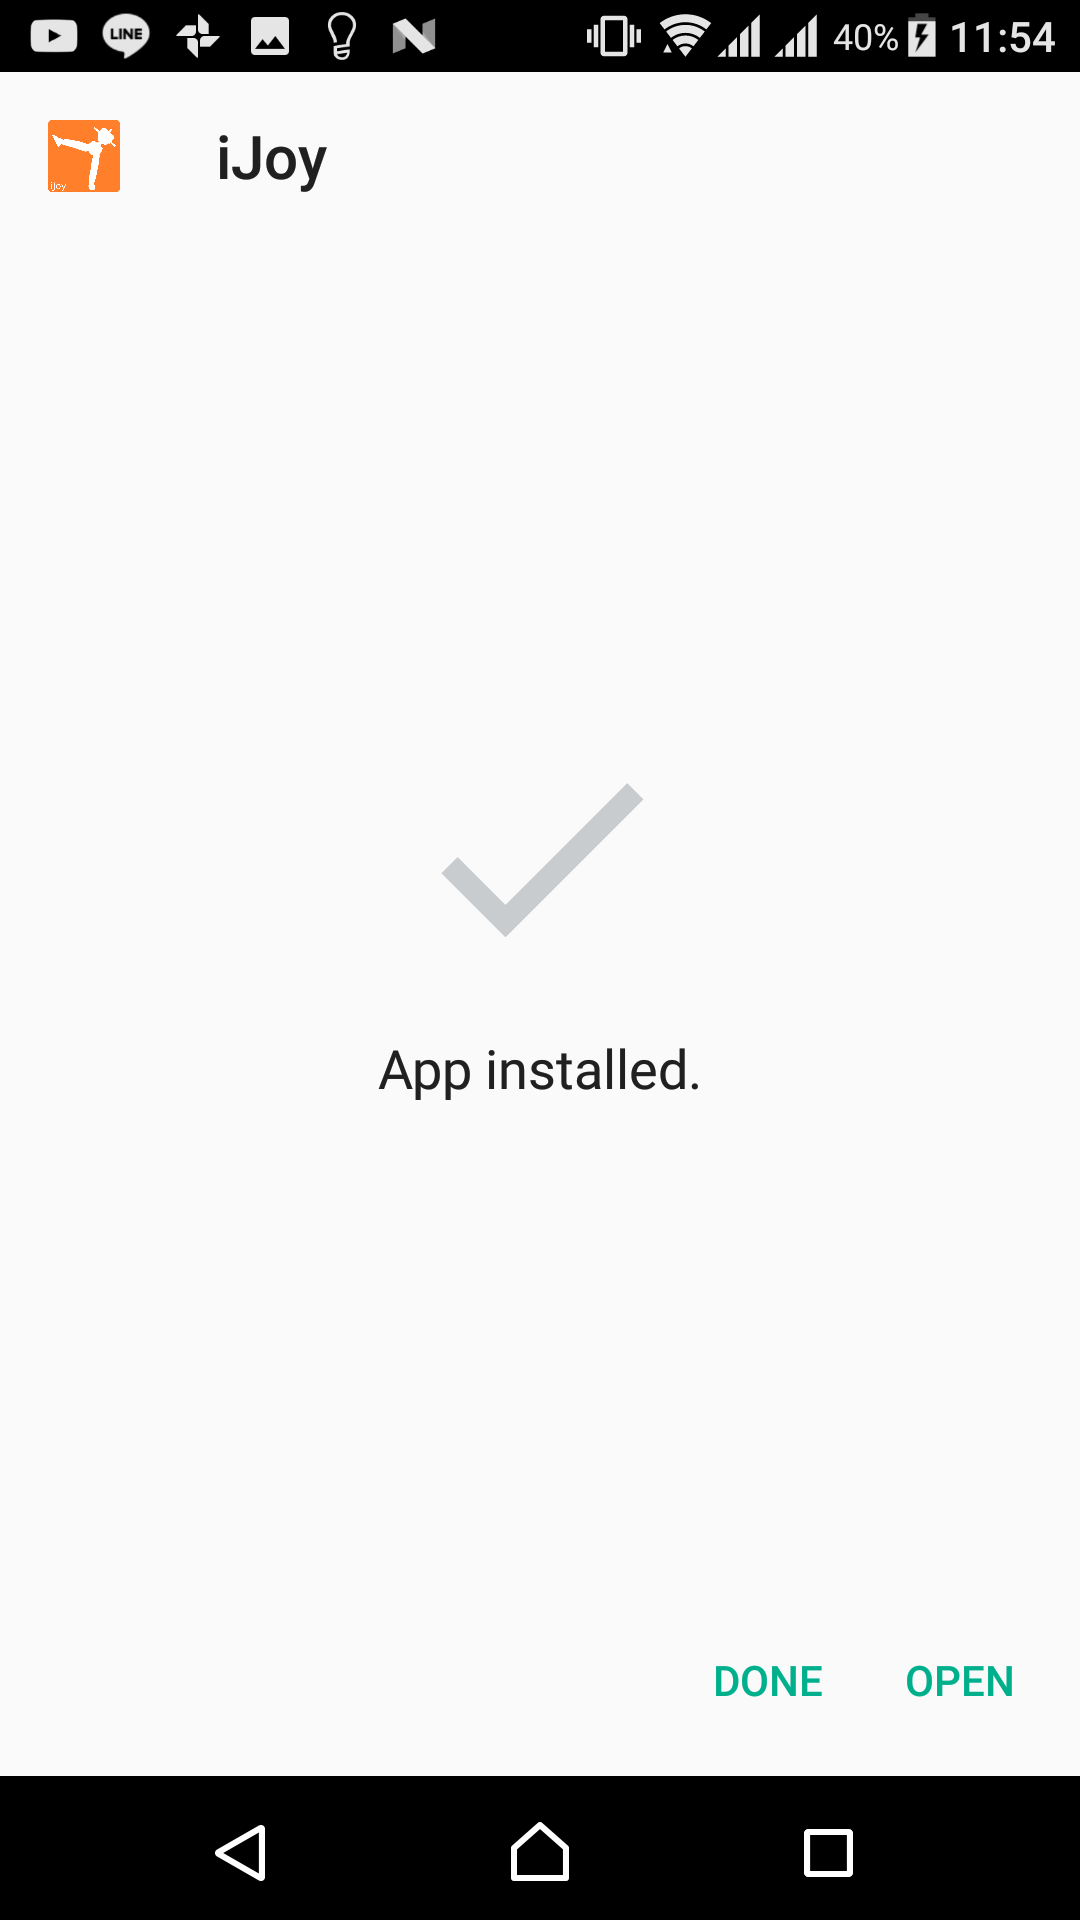
\includegraphics[scale=.06]{chapters/07_appendix/img/installation_end.png}}
		\caption{Installation process.}
		\label{fig::A2_apk}
	\end{figure}
	\item Follow the on screen instructions and wait for the installation to finish (figure \ref{fig::A2_apk} (c) and (d)).
\end{enumerate}
\section{Build Proximal Policy Optimization}
The proximal policy optimization can be found on GitHub at the following \href{https://github.com/mhubii/ppo_libtorch}{link}. Proceed as described below.
\begin{enumerate}
	\item Make sure the C++ API of PyTorch got install as described in section \ref{sec::A5_tp}.
	\item Clone proximal policy optimization from GitHub with
	\newline \inlinecode{}{git clone https://github.com/mhubii/ppo_libtorch.git}
	\item Then do
	\newline \inlinecode{}{mkdir build \&\& cd build}
	\newline \inlinecode{}{cmake -DCMAKE\_PREFIX\_PATH=/absolute/path/to/libtorch ..}
	\newline \inlinecode{}{make}
\end{enumerate}
You can then train and evaluate the neural network as described below.
\begin{enumerate}
	\item Train the neural network with
	\newline \inlinecode{}{cd build}
	\newline \inlinecode{}{./train\_ppo}
	\item Test the trained neural network with
	\newline \inlinecode{}{cd build}
	\newline \inlinecode{}{./test\_ppo}
	\item Visualize the results with
	\newline \inlinecode{}{python plot.py}
\end{enumerate}
\section{Build Simulation Models}
\label{sec::A4_sm}
The simulation models can be found on GitHub at the following \href{https://github.com/mhubii/gazebo_models/}{link}. Proceed as described below.
\begin{enumerate}
	\item Clone the models from GitHub with
	\newline \inlinecode{}{git clone https://github.com/mhubii/gazebo_models.git}
	\item You can either install the models to a location that Gazebo knows, or update the path, where Gazebo is looking for models.
	\item To update the path add following line to your \inlinecode{}{bashrc}
	\newline \inlinecode{}{export GAZEBO\_MODEL\_PATH=<>/gazebo\_models:\$GAZEBO\_MODEL\_PATH}
	\newline Therein, replace \inlinecode{}{<>} by the location to which you cloned the repository.
	\item To install the models do
	\newline \inlinecode{}{mkdir build \&\& cd build}
	\newline \inlinecode{}{cmake -DCMAKE\_INSTALL\_PREFIX=~/.gazebo ..}
	\newline \inlinecode{}{make install}
	\item To uninstall the models do
	\newline \inlinecode{}{cd build}
	\newline \inlinecode{}{make uninstall}
\end{enumerate}
\section{Build Third Party Software}
\label{sec::A5_tp}
